\documentclass[border=12pt]{standalone}
\usepackage{tikz}
\usetikzlibrary{arrows.meta,positioning,fit,calc}
\usepackage{fontspec}

\definecolor{bgpage}{HTML}{F7F8FA}
\definecolor{offlinebg}{HTML}{EEF2F7}
\definecolor{onlinebg}{HTML}{F0F7F4}
\definecolor{docfill}{HTML}{E8EDF5}
\definecolor{docborder}{HTML}{5B6B8A}
\definecolor{embedfill}{HTML}{E4ECF8}
\definecolor{embedborder}{HTML}{3D6BB3}
\definecolor{vdbfill}{HTML}{EDE8F8}
\definecolor{vdbborder}{HTML}{6B4FA0}
\definecolor{queryfill}{HTML}{E6F4EF}
\definecolor{queryborder}{HTML}{2A8F6F}
\definecolor{retrfill}{HTML}{E8F0FA}
\definecolor{retrborder}{HTML}{2F6FBF}
\definecolor{ctxfill}{HTML}{FFF6E8}
\definecolor{ctxborder}{HTML}{C4842A}
\definecolor{llmfill}{HTML}{FCECE8}
\definecolor{llmborder}{HTML}{C24A3A}
\definecolor{ansfill}{HTML}{E8F6EC}
\definecolor{ansborder}{HTML}{2E8B57}
\definecolor{labelfg}{HTML}{3A4556}
\definecolor{arrowc}{HTML}{5A667A}
\definecolor{titlefg}{HTML}{1F2A3A}

\begin{document}
\pagecolor{bgpage}
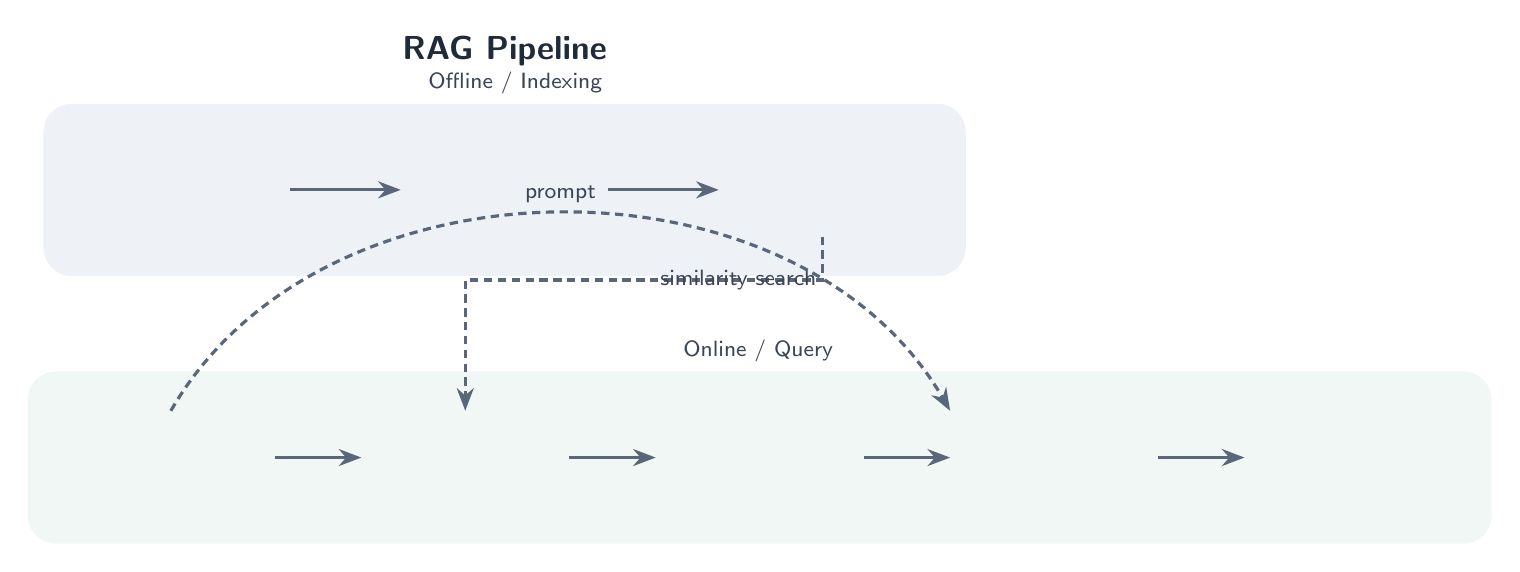
\begin{tikzpicture}[
  font=\sffamily\small,
  >=Stealth,
  box/.style={
    draw=#1,
    fill=#1!12,
    line width=1.1pt,
    rounded corners=5pt,
    align=center,
    minimum width=2.6cm,
    minimum height=1.15cm,
    inner sep=6pt,
    text=titlefg
  },
  zone/.style={
    draw=#1,
    fill=#1,
    rounded corners=10pt,
    inner sep=14pt
  },
  arr/.style={
    ->,
    line width=1.15pt,
    draw=arrowc
  },
  lbl/.style={
    font=\sffamily\footnotesize,
    text=labelfg
  }
]

% --- Offline zone (top) ---
\node[box=docborder, fill=docfill] (docs) at (0,4.2) {Documents\\Corpus};
\node[box=embedborder, fill=embedfill, right=1.4cm of docs] (chunk) {Chunk\\\& Embed};
\node[box=vdbborder, fill=vdbfill, right=1.4cm of chunk] (vdb) {Vector DB\\(Index)};

\node[zone=offlinebg, fit=(docs)(chunk)(vdb),
  label={[lbl,anchor=south west]above left:{Offline / Indexing}}] (offzone) {};

\draw[arr] (docs) -- (chunk);
\draw[arr] (chunk) -- (vdb);

% --- Online zone (bottom) ---
\node[box=queryborder, fill=queryfill] (query) at (-0.2,0.8) {User Query};
\node[box=retrborder, fill=retrfill, right=1.1cm of query] (retr) {Embed\\\& Retrieve};
\node[box=ctxborder, fill=ctxfill, right=1.1cm of retr] (ctx) {Retrieved\\Context};
\node[box=llmborder, fill=llmfill, right=1.1cm of ctx] (llm) {LLM};
\node[box=ansborder, fill=ansfill, right=1.1cm of llm] (ans) {Answer};

\node[zone=onlinebg, fit=(query)(retr)(ctx)(llm)(ans),
  label={[lbl,anchor=south west]above left:{Online / Query}}] (onzone) {};

\draw[arr] (query) -- (retr);
\draw[arr] (retr) -- (ctx);
\draw[arr] (ctx) -- (llm);
\draw[arr] (llm) -- (ans);

% Vector DB feeds retrieval (cross-zone)
\draw[arr, densely dashed]
  (vdb.south) -- ++(0,-0.55) -| (retr.north)
  node[pos=0.25,lbl,right=2pt] {similarity search};

% Query also informs LLM (optional context path label)
\draw[arr, densely dashed, bend left=18]
  (query.north) to[out=60,in=120]
  node[midway,lbl,above] {prompt}
  (llm.north west);

% Title
\node[font=\sffamily\large\bfseries, text=titlefg, above=0.35cm of offzone.north]
  {RAG Pipeline};

\end{tikzpicture}
\end{document}
